%!TEX root = ../main.tex

\chapter{SoundRise: the Background Idea}
\label{chp:background}

\paragraph{}
This chapter explains the fundamental concept and overall functionality of the SoundRise application, detailing its past versions. Specifically, a focus will be placed on its reactivation based on models studied and defined inside the CSC (Centro di Sonologia Computazionale), and the procedural aspects of applying reactivation to SoundRise will be delineated.

\section{What is SoundRise}
\label{sec:what-is-soundrise}

\paragraph{}
SoundRise is an innovative educational game designed to support children in discovering and understanding their vocal abilities. It serves as a complementary tool to traditional speech therapy, offering an engaging and interactive platform for autonomous learning. The application is particularly beneficial for children with hearing impairments, providing them with a unique opportunity to explore their vocal capabilities in a supportive environment.

\paragraph{}
The core aim of SoundRise, since its inception about 10 years ago, has been to create an interactive application that utilizes real-time analysis of vocal features. This approach helps children understand how their voice works by providing immediate visual feedback. The application employs advanced audio processing techniques to analyze vocal input, allowing users to see a graphical representation of their voice in real-time.

\paragraph{}
SoundRise is particularly focused on helping deaf children acquire a deep understanding of their vocal capabilities. The application uses a playful metaphor of a sleeping sun that reacts to the child's voice. When the sun hears a sound, it opens its eyes and changes its appearance and position. This visual feedback is crucial for children to monitor their progress and make necessary adjustments to their vocal output.

\paragraph{}
The sun's movements are directly linked to the vocal input: it rises and falls vertically according to the pitch of the sound emitted, grows bigger or smaller depending on the sound intensity, and changes color based on the vocal timbre detected. This color change is associated with the identification of the five vowels of the Italian language, with each vowel corresponding to a different color of the sun. This innovative approach not only makes learning fun but also enhances the child's ability to recognize and produce different vowel sounds.



\paragraph{}
In Figure 3.1, the first interface of the SoundRise application, developed by Stefano Giusto \cite{giusto2012} in Pure Data, is shown. This interface, running on a PC in the CSC, laid the foundation for subsequent developments and improvements in the application, as detailed in the following sections.


\paragraph{}
The child's voice is interpreted by a sleeping sun. When the sun hears a sound (i.e. when the microphone recognises a sound), it opens its eyes and changes its appearance and position. The change of the sun depends on the changing sound expressed by the child's voice. The sun can rise and fall vertically according to the pitch of the sound emitted. It can grow bigger or smaller depending on the sound intensity. The sun also changes its colour, based on the vocal timbre detected. The recognition of this property is related to the identification of the five vowels of the Italian language: graphically, each possible timbre (5, as the vowels) corresponds to a different colour of the sun.

\paragraph{}
By providing a visual representation of the emitted sound, SoundRise helps children correct their pronunciation and improve their vocal skills. The application is designed to be intuitive and user-friendly, ensuring that even young users can navigate it with ease. The engaging interface and immediate feedback make it an effective tool for speech therapy, encouraging children to practice and improve their vocal abilities.

\paragraph{}
Therefore, the application uses the user's vocal input to create an interactive visual experience, providing to the child a visual feedback on the emitted sound of his/her voice, helping him/her to correct himself/herself, with the aim of educating him/her in the use of his/her own voice.

\paragraph{}
In Figure 3.1 it is possible to see the first interface of the SoundRise application, developed by Stefano Giusto \cite{giusto2012} in Pure Data (more details in the next sections) that is running on a PC in the CSC.

\begin{figure}[h]
    \centering
    \includegraphics[width=0.8\textwidth]{res/images/background/soundrise-1.png}
    \caption{First interface of the SoundRise application}
    \label{fig:soundrise-logo}
\end{figure}

\section{The Evolution of SoundRise Over Time}
\label{sec:evolutionOfSoundRise}

\paragraph{}
The first idea for SoundRise was sketched out by Prof. Federico Avanzini, Prof. Antonio Rodà and Prof. Sergio Canazza from the Department of Information Engineering at the University of Padua, in collaboration with Dr. Serena Zanolla from the University of Udine. From then on, the project started to develop in the CSC (Centro di Sonologia Computazionale) at the University of Padua.

\paragraph{}
The initial development of SoundRise was carried out through three significant master thesis projects at the University of Padua. In 2012, two foundational theses were completed: Stefano Giusto's work (Giusto S. Rodà A., SoundRise: Studio e Progettazione Di un'Applicazione Multimodale Interattiva Per La Didattica Basata sull'Analisi Di Feature Vocali) \cite{giusto2012} and Marco Randon's research (Randon M. Avanzini F., SoundRise: Sviluppo E Validazione Di un'Applicazione Multimodale Interattiva Per La Didattica Basata Sull'analisi Di Feature Vocali) \cite{randon2012}. More recently, in 2023, Giada Zuccolo's thesis "A New Sunrise for Speech Therapy: Development of SoundRise 2.0 Application" \cite{zuccolo2023} brought significant advancements to the project, focusing on modernizing the application and enhancing its therapeutic capabilities.

\paragraph{}
These three master theses collectively established and evolved SoundRise as a comprehensive educational-therapeutic tool. The initial versions developed by Giusto and Randon laid the foundation as a standalone application aimed at supporting vocal therapy and voice modulation practice for young users. Zuccolo's recent contribution further enhanced the system by implementing new features and improving the user experience for both therapists and children.

\paragraph{}
In the master thesis of Stefano Giusto \cite{giusto2012}, the application was developed using the real-time graphical programming environment Pure Data\footnote{Pure Data (Pd) is an open source visual programming language for multimedia.} \cite{puredata2015} and the external library timbreID for vocal timbre analysis. timbreID \cite{timbreid2016} represents a collection of externals for Pd, developed by William Brent. The features generated through the external objects can be used directly as control information in real-time performance. This library consists of a group of objects for extracting timbre features and a classification object that manages the resulting database of information. The incoming audio signal is processed by a specific object that detects attacks, defined as abrupt changes in the spectral envelope of the incoming sound, and generates a maximum match relation.

\paragraph{}
Subsequently, in the master thesis of Marco Randon \cite{randon2012}, the application was modified to enhance its portability across different platforms. To achieve this, it became necessary to modify its architecture in a manner that would allow it to run independently of Pd while maintaining its core features and functionalities. Moreover, efforts were made to improve its graphical interface to adapt it for touchscreen devices. This new version of the application was developed in C++ language and using the libpd library for the communication with Pd. In essence, libpd consists of variations of processing callback functions for different sample types, a set of functions for sending messages to Pd, and a series of function pointers for receiving messages from Pd. In order to receive messages, the client code must implement the appropriate receive functions and assign them to the corresponding function pointers in libpd.

\paragraph{}
libpd includes language wrappers (C++, and others) that make libpd's functionality available to the respective programming language. These wrappers perform data type conversions between Pd's custom data types and the standard data types of the target language. They provide an object-oriented interface for message exchange functions and function pointers. To receive messages from Pd, the client code must implement the necessary methods of the PdReceiver interface and register a receiver object using the methods of the PdBase class.

\paragraph{}
A more detailed study of the functioning of SoundRise was carried out by Riccardo Fila (Canazza Targon S., Fiordelmondo A., Fila R., SoundRise 2.0: Sviluppo di un modello di riconoscimento timbrico per un sistema di assistenza web dedicato a persone con disabilità uditive) \cite{fila2020}. In this thesis, that is the last project related with SoundRise before this thesis, an in-depth study was carried out in order to develop a timbre recognition model. This project was developed in Javascript with the aid of Web Audio API (explained in detail in the chapter 4, on the section 4.2). Basically, a function calculates the first two formant frequencies of the voice and compares them with those characteristic of Italian vowels in order to find an effective match and display it graphically. The idea of developing this type of application on the web was a turning point, as will be explained in Chapters 4 and 5, mainly because of the possibility of being able to exploit the potential of the Web Audio API.

\paragraph{}
In Figure 3.2, it is possible to see the interface of this prototype, so how it works: after starting the microphone, it analyses voice data and shows the resulting vowel (when it is able to capture it): the yellow column shows the vowel that was recognised by the model (if it was recognised), while the subsequent green columns show the analysed frequency values.

\begin{figure}[h]
    \centering
    \includegraphics[width=0.8\textwidth]{res/images/soundrise-1.png}
    \caption{SoundRise web prototype interface}
    \label{fig:soundrise-1}
\end{figure}



\paragraph{}
The formant frequencies play a crucial role in vowel recognition within the Italian language system. Each vowel has its distinct characteristic formant frequencies that serve as acoustic signatures. For the vowel /a/, the first formant (F1) typically occurs around 800Hz, while the second formant (F2) is found near 1400Hz, creating its characteristic open sound. The vowel /e/ exhibits F1 at approximately 400Hz and F2 at 2000Hz, producing its mid-front quality. The high front vowel /i/ is characterized by a low F1 of about 250Hz and a high F2 of 2250Hz. The back vowel /o/ shows F1 around 400Hz and F2 near 800Hz, while /u/ has F1 at approximately 250Hz and F2 at 600Hz, creating its distinctive high back quality.

\paragraph{}
The duration of vowel sounds represents another critical parameter in speech analysis and recognition. In natural speech, Italian vowels typically range from 100 to 300 milliseconds in duration. This duration can vary significantly based on factors such as speaking rate, stress patterns, and phonetic context. In stressed positions, vowels tend toward the longer end of this range, while unstressed vowels are generally shorter. This temporal characteristic provides important cues for both speech recognition systems and human listeners.

\paragraph{}
Intensity patterns also serve as distinctive features for vowel identification. Each vowel exhibits characteristic amplitude patterns that contribute to its unique acoustic profile. These patterns are influenced by the specific configuration of the vocal tract during production and play a crucial role in vowel perception. High vowels like /i/ and /u/ typically show lower intrinsic intensity compared to low vowels like /a/, due to physiological factors in their production. Understanding these intensity patterns is essential for developing accurate vowel recognition systems.

\paragraph{}
These acoustic parameters - formant frequencies, duration, and intensity - form the foundation of vowel recognition in SoundRise. The application's analysis system carefully monitors these characteristics in real-time, enabling accurate identification of the produced vowels and providing appropriate visual feedback through the sun interface. This comprehensive approach to vowel analysis ensures reliable recognition across different speakers and speaking conditions.

\section{SoundRise 2.0: A New Era}
\label{sec:soundrise-2}

\paragraph{}
The most recent and significant evolution of SoundRise came through Giada Zuccolo's master thesis "A New Sunrise for Speech Therapy: Development of SoundRise 2.0 Application" \cite{zuccolo2023}, supervised by Professor Sergio Canazza Targon and co-supervised by Dott. Alessandro Fiordelmondo. This work represents a fundamental shift in the application's architecture and capabilities, establishing the foundation for modern speech therapy applications.

\paragraph{}
SoundRise 2.0 introduced a complete architectural overhaul, moving away from the traditional standalone application model to a modern web-based architecture. The application was rebuilt using React.js for the frontend, providing a responsive and intuitive user interface. The backend implementation utilized Python, enabling robust audio processing and analysis capabilities. This architectural decision significantly improved accessibility and maintainability while facilitating future enhancements.

\begin{figure}[h]
    \centering
    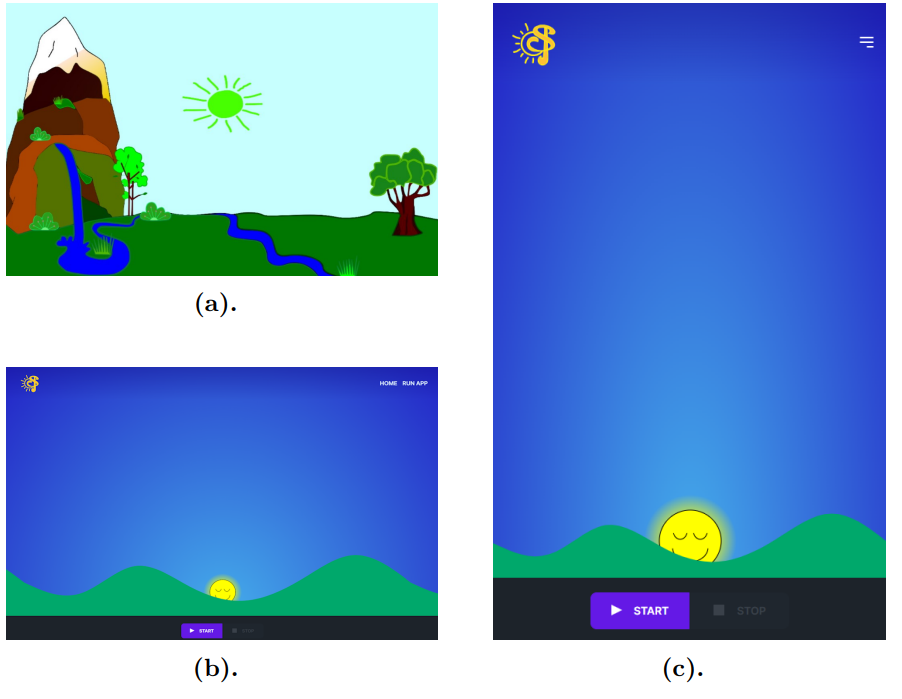
\includegraphics[width=0.8\textwidth]{res/images/background/soundrise-2.png}
    \caption{SoundRise web prototype interface}
    \label{fig:soundrise-2}
\end{figure}

\paragraph{}
The new version brought substantial improvements to the user interface, maintaining the engaging sun metaphor while introducing more sophisticated visual feedback mechanisms. The interface was designed with particular attention to the needs of young users and speech therapists. At its core, the application features intuitive controls for audio recording and playback, ensuring that even young users can easily navigate and interact with the system. The real-time visual feedback system provides immediate response to vowel pronunciation, helping users understand and correct their articulation patterns. Progress tracking has been enhanced with clear indicators and achievement metrics, allowing both users and therapists to monitor improvement over time. The responsive design ensures optimal functionality across various device sizes, making the application accessible in different therapeutic settings.


\paragraph{}
Zuccolo's implementation brought several significant technical improvements to the platform. The integration of the Web Audio API enables precise audio capture and analysis, providing the foundation for accurate vowel recognition. Advanced audio processing algorithms were implemented to enhance the quality and reliability of speech analysis. The addition of real-time spectrogram generation and analysis provides detailed insights into vowel pronunciation patterns. The formant analysis system was significantly improved, leading to more accurate vowel recognition across different speakers and acoustic conditions.


\paragraph{}
SoundRise 2.0 was developed with a strong focus on clinical applicability, incorporating features essential for therapeutic use. The application supports structured therapy sessions through a carefully designed progression of exercises and activities. A comprehensive progress tracking system allows therapists to monitor and document patient improvement over time. The platform enables customization of exercises based on individual patient needs and therapeutic goals. Additionally, the system facilitates effective communication between therapists and patients, creating a collaborative environment for speech therapy.


\paragraph{}
Zuccolo's work on SoundRise 2.0 has established a robust foundation for future developments in speech therapy applications. The modular architecture and modern technology stack enable continuous improvement and feature expansion. This version serves as the basis for subsequent research and development, including the current work on implementing CNN-based vowel recognition systems, which aims to further enhance the application's accuracy and effectiveness in speech therapy settings.

\paragraph{}
The success of SoundRise 2.0 in combining technical innovation with clinical utility has opened new possibilities for computer-aided speech therapy. The application demonstrates how modern web technologies and thoughtful design can create effective tools for speech therapy, particularly for children with hearing impairments. This foundation continues to evolve through ongoing research and development efforts at the University of Padua.

\section{Summary}
\label{sec:summary}

\vspace{0.5cm}

\paragraph{}
This chapter has provided an in-depth look at the SoundRise application, detailing its origins, core functionalities, and the innovative methodologies it employs to support speech therapy. SoundRise's unique approach, using real-time visual feedback through a playful sun metaphor, has proven effective in helping children, particularly those with hearing impairments, to explore and improve their vocal abilities. The chapter also highlighted the technological advancements and educational benefits that SoundRise offers, setting the stage for its continued evolution and impact in the field of speech therapy. This comprehensive overview underscores the significance of SoundRise as a tool for enhancing vocal learning and therapy.



